%\documentclass[12pt, draftclsnofoot, onecolumn,letterpaper]{IEEEtran}
\documentclass[12pt, letterpaper]{article}
%\documentclass[12pt, letterpaper]{IEEEtran}
\usepackage{ multirow }
\usepackage{longtable}
\usepackage{geometry}
\usepackage{ragged2e}
\usepackage[table]{xcolor}
\usepackage{booktabs}
\usepackage{graphicx}
\usepackage{caption}
\usepackage{subcaption}
\usepackage{lipsum}
\usepackage{makeidx}
\usepackage{enumerate}
\usepackage{color}
\usepackage{refstyle}
\usepackage{cite}
\usepackage{amsmath}
\usepackage{amssymb}
\usepackage{nomencl}
\usepackage{amsmath}
\usepackage{multirow}
\usepackage{graphicx}
\usepackage{multirow}
\usepackage{anysize}
\usepackage{float}
\usepackage{epstopdf}
\usepackage{threeparttable}
\usepackage{multicol}
\usepackage{amssymb}
\usepackage{adjustbox}
\usepackage{hyperref}
%\usepackage[none]{hyphenat}
%\usepackage{float}

%\usepackage{fixltx2e}
\usepackage{amsmath, amssymb, upgreek, amsthm}
\usepackage{graphicx}
\usepackage{tikz}
\geometry{letterpaper, left=20mm, right=20mm, top=20mm, bottom=20mm}
\usetikzlibrary{patterns} % LATEX and plain TEX when using Tik Z
\allowdisplaybreaks
\setlength{\textfloatsep}{2ex}
\usepackage{array}
\usepackage{enumitem}
\setlength{\parindent}{1 em}
\setlength{\parskip}{0.5 em}
\renewcommand{\baselinestretch}{1.25}
\def\dsd{d_\text{SD}}
\def\Rcoop{R_\text{Coop}}
\def\rhd{R_\text{HD}}
\def\rsd{R_\text{SD}}
\def\rsh{R_\text{SH}}
\def\Pcoops{\mathcal{P}^\text{Succ}_\text{Coop}}
\def\dsh{d_\text{SH}}
\def\dhd{d_\text{HD}}
\def\psibar{\overline{\mathcal{P}}^\text{Succ}_{i}}
\def\psbara{\overline{\mathcal{P}}^\text{Succ}_{1}}
\def\psbarb{\overline{\mathcal{P}}^\text{Succ}_{2}}
\def\psbarc{\overline{\mathcal{P}}^\text{Succ}_{3}}
\def\psbard{\overline{\mathcal{P}}^\text{Succ}_{4}}
\def\psbare{\overline{\mathcal{P}}^\text{Succ}_{5}}
\def\Ri{R_{i}}
\def\Ps{\mathcal{P}^\text{Succ}_\text{Direct}}
\def\frk{\mathrm{f}_{r_k}(r)}
\def\Rcoopj{R_\text{coop}^j}
\title{\bf \vspace*{-4ex} Statement of Responses to the Editor and the Reviewers of Paper-TNSM \\[-6ex]}
\date{}

\begin{document}
%\vspace*{-10ex}
%\sloppy
\maketitle
We would like to thank the editor and reviewers for their constructive comments on our manuscript. They have been beneficial in revising this paper, and we have improved the technical content and presentation quality through their assistance. We greatly appreciate their generous help. In addition, we would like to acknowledge the assistance of Dr. Onel Luis Alcaraz López in this revision.
Moreover, we have reviewed and incorporated all the comments and suggestions.
We hope that the modifications we have made to the manuscript and the responses we have provided herein will alleviate the reviewers' concerns. Below, please find our detailed responses to the editor and reviewers' comments and suggestions.
\\ [-3.ex]
% % % % % % % % % % % % % % % Editor % % % % % % % % % % % % % % % % % % % %


\clearpage
\noindent
\begin{longtable}{|p{0.975\textwidth}|}
\hline \hline
\Centering
\cellcolor{gray!60}
\textbf{Editor} \\
\hline \hline %\hline \hline \hline
\RaggedRight
\cellcolor{violet!15}
\textbf{\noindent  Comments to the Author} ``I think the paper should undergo a major revision. It is important to take special attention to the comments of reviewer 2.''\\
\hline
\end{longtable}

\vspace*{-1\baselineskip}
\noindent \textbf{Response:\\}
We would like to thank the Editor for his comments and for giving us this opportunity to improve our paper. We have used the comments to improve our paper and eliminate problems.

%\begin{longtable}{|p{0.975\textwidth}|}
%\hline \hline
%\RaggedRight
%\cellcolor{green!10}
%[1] F. Patolsky, B. P. Timko, G. Yu, Y. Fang, A. B. Greytak, G. Zheng, and C. M. Lieber, ``Detection, stimulation, and inhibition of neuronal signals with high-density nanowire transistor arrays,'' Science, vol. 313, no. 5790, pp. 1100-1104, 2006.
%\\
%\hline
%\end{longtable}




% % % % % % % % % % % % % % % Reviewer 1 % % % % % % % % % % % % % % % % % % % %
\clearpage
\noindent
\begin{longtable}{|p{.975\textwidth}|}
\hline \hline %\hline \hline \hline
\Centering
\cellcolor{gray!60}
\textbf{Reviewer 1} \\
\hline \hline %\hline \hline \hline
\RaggedRight
\cellcolor{violet!15}
\textbf{\noindent Comments to the Author} ``
The authors have addressed the comments provided in a previous review. The contributions are clear and the results are compared to some related work, so the reader can somewhat contextualize the proposed solution. ''\\
\hline
\end{longtable}
\vspace*{-1\baselineskip}
\noindent \textbf{Response:\\}
We would like to thank the reviewer for the careful and thorough reading of this manuscript. We hope that the responses provided herein can alleviate the reviewer's concerns.

\begin{longtable}{|p{0.975\textwidth}|}
\hline \hline
\RaggedRight
\cellcolor{gray!15}
\textbf{\noindent Comment1:} ``However, the paper still needs some improvement in terms of readability. Some paragraphs are too long  ''\\
\hline
\end{longtable}
\vspace*{-1\baselineskip}
\noindent \textbf{Response:\\}
We revised the whole paper and checked the text entirely according to this comment. For instance, the introduction has been rewritten totally. We also revised the system model, proposed algorithms too, and shortened long paragraphs based on these comments. Moreover, we shortened the numerical results and feasible region section, and modified the conslusion section.  
\begin{longtable}{|p{0.975\textwidth}|}
\hline \hline
\RaggedRight
\cellcolor{gray!15}
\textbf{\noindent Comment2:} `` the figures are difficult to locate from their reference in the text (figures at top, as typical IEEE template is better), the text in the figures is too small ''\\
\hline
\end{longtable}
\vspace*{-1\baselineskip}
\noindent \textbf{Response:\\}
Thank you for this comment. We think that these changes improve the readability of the manuscripts.
 We modified all the paper's figures entirely concerning this comment and located them in sub-figures to make them more determined. Moreover, we modified whole the figures and made the texts larger and more readable. 
\begin{longtable}{|p{0.975\textwidth}|}
\hline \hline
\RaggedRight
\cellcolor{gray!15}
\textbf{\noindent Comment3:} ``the contributions discussed in the introduction are not easily found in the other parts of the paper.  ''\\
\hline
\end{longtable}
\vspace*{-1\baselineskip}
\noindent \textbf{Response:\\}
We thank the reviewer for asking us to add clarity to our paper and reducing ambiguity in this condition.  We changed the contribution in a better way based on this comment. We have removed some sentences and rewritten the contributions in the same order of our paper's section.
Below we report the whole contribution section.


This paper aims to optimize the resource utilization of a downlink O-RAN system to develop an isolated network slicing outline for the three 5G service classes.
We use mathematical methods to decompose and convexify the problem and solve it using hierarchical algorithms.
%Our paper focuses on the multi-service resource management of the RAN slicing in an open and flexible O-RAN architecture.}
%In this paper, as depicted in Figure \ref{fig:c11}, the downlink of the O-RAN system is studied.
 The main contributions of this paper are summarized as follows:
\begin{itemize}
\item We examine the problem of radio resource allocation and VNF activation within the O-RAN architecture.
Based on the three types of 5G service classes, i.e., eMBB, URLLC and mMTC, and their corresponding QoS requirements and service priorities, we formulate a problem for allocating baseband resources such as power, physical resource blocks (PRBs), O-RUs, and activating VNFs to maximize the weighted throughput of the O-RAN.
\item We propose a two-step resource management algorithm for solving the optimization problem.
In the first step, we reformulate and simplify the problem so as to find an upper and lower bound for the number of activated VNFs. Moreover, we use the Lagrangian function and Karush-Kuhn-Tucker (KKT) conditions to obtain the optimal power and PRB allocation. In the second step, the problem of O-RU association is converted to a multiple knapsack problem and solved by a greedy algorithm.
\item We provide insights into the complexity of the proposed algorithms and demonstrate their convergence. Additionally, we analyze the feasibility region of the problem under consideration and introduce a fast algorithm to check its feasibility numerically.
\item We show via numerical results that the proposed algorithm outperforms two baseline schemes in terms of achievable data rate and mean total delay. Remarkably, the proposed algorithm performs close to the optimal solution in low-interference conditions.
\end{itemize}

% % % % % % % % % % % % % % % Reviewer 2 % % % % % % % % % % % % % % % % % % % %
\clearpage
\noindent
\begin{longtable}{|p{.975\textwidth}|}
\hline \hline %\hline \hline \hline
\Centering
\cellcolor{gray!60}
\textbf{Reviewer 2} \\
\hline \hline %\hline \hline \hline
\RaggedRight
\cellcolor{violet!15}
\textbf{\noindent Comments to the Author} ``
The Reviewer would like to thank the authors for their revision of the paper with respect to the comments and suggestions in the previous submission. Whereas the authors have considered parts of the suggestions and improved specific areas of the work, there are still a lot of remaining issues of concern in the current version of the paper. ''\\
\hline
\end{longtable}
\vspace*{-1\baselineskip}
\noindent \textbf{Response:\\}
It is our pleasure to thank the reviewer for the careful reading of this manuscript, providing
thoughtful comments, and offering constructive suggestions that strengthened and enhanced its
quality. We hope that the responses provided herein can alleviate the reviewer’s concerns.

\begin{longtable}{|p{0.975\textwidth}|}
\hline \hline
\RaggedRight
\cellcolor{gray!15}
\textbf{\noindent Comment1:} ``While the authors have taken into consideration the Reviewer’s comments about the re-structuring of the Introduction, I am afraid that the current version is not in the adequate state for publication. Initially, the paragraphs of the Introduction have no logical connection among them. It seems that until the Related Literature subsection all paragraphs are disconnected and only introduce concepts. ''\\
\hline
\end{longtable}
\vspace*{-1\baselineskip}
\noindent \textbf{Response:\\}
As suggested by the reviewer, we modified the introduction completely. The final version is reported below.


\section{Introduction}
%\subsection{State Of The Arts}
Network slicing is a key technology in 5G wireless systems. Specifically, network slicing provides the isolation of network resources into slices, e.g., via core slicing and/or radio access network (RAN) slicing, for serving multiple and heterogeneous service classes [1]–[3]. There are three main service classes in 5G, namely enhanced mobile broadband (eMBB), ultra-reliable low latency communications (URLLC), and massive machine-to-machine communications (mMTC). Depending on their corresponding quality of service (QoS) requirements, each service is assigned to a slice of the network.
For instance, the eMBB service demands high capacity and throughput,  e.g., 8K video streaming and immersive gaming. Meanwhile, the URLLC service, leveraged, e.g., by autonomous vehicles, Tactile Internet, and remote surgery services, is concerned with providing ultra-reliable and low-latency connectivity. Finally, mMTC services require connectivity for a large number of Internet of Things (IoT) devices that transmit small payloads  [4]–[6].
%\cite{dogra2020survey,kassab2018coexistence,alsenwi2021intelligent,SL}.}

Unfortunately, the existing radio access network (RAN) architecture still lacks adequate flexibility and openness to manage these demands for various services simultaneously. In view of this, a new RAN paradigm, called open RAN (O-RAN), which is schematically represented in Fig. 1, is introduced to deal with these issues.
%This paper considers several user equipments (UEs) requesting one of these types of services with different QoS in the O-RAN architecture. We want to study RAN slicing technology and the isolation between slices in this system to evaluate the performance of various services.
%This paper aims to design a RAN slicing technology for the O-RAN architecture. 
%O-RAN offers machine learning techniques based on the requirement for an intelligent wireless network for the next generation of RAN systems. The two logical nodes, RIC-Non Real-Time (which is placed in Orchestration and Automation node) and RIC-Near Real-Time, implement the algorithms for network intelligence

A key feature of the O-RAN architecture is that the hardware is disaggregated from the software, leading to network function virtualization (NFV). Additionally, each component is implemented as a virtual network function (VNF), the system function block in NFV, that can be deployed on a virtual machine (VM) or container [7].
As a result, some O-RAN components defined in Section III, such as user plane function (UPF), O-RAN central unit (O-CU), O-RAN distributed unit (O-DU), and RAN intelligent controller (RIC)-near real-time, are virtualized and implemented as VNFs.

\subsection{Motivation}
The problem of finding the optimal resource allocation, independently of the specific RAN technology, is vital for reducing the cost of the system and improving the QoS of the user equipments (UEs). In case of 5G systems, there are many related significant challenges such as interference alignment, limited capacity of fronthaul links, energy restrictions on virtual machines, etc [2], [8], [9]. 

Many studies have investigated resource allocation in cloud RAN (C-RAN) by considering the power, data rate and delay limitations of a single service. Due to the contemporary need to serve services with different QoS simultaneously, e.g., as in 5G and beyond, this architectural model is inefficient. In this regard, the O-RAN architecture has emerged as a flexible, layered, and modular design architecture that can simultaneously support multiple services at a lower cost. Nevertheless, RAN slicing in the O-RAN architecture still faces various challenges. 
One of the fundamental problems lies in attaining a balance between different services with different QoS, resource requirements, and priorities [1], [10]–[12].  
%\textcolor{MidnightBlue}{Since 5G defines different services with different QoS, we need to analyze the resource allocation for each 5G service, using RAN slicing to guarantee the QoS for them.
%Consequently, we consider the O-RAN architecture, the new generation of RAN architecture that can implement RAN slicing for different 5G services. 
%We investigate the problem of resource allocation in the O-RAN architecture for the three services defined in the 5G with different QoS serving simultaneously.}

The purpose of this paper is to design a system in the O-RAN architecture to support the three types of 5G services, namely, eMBB, URLLC, and mMTC via network slicing and resource allocation. Specifically, we aim to maximize the total achievable data rate and satisfy the minimum achievable data rate for eMBB services while meeting the URLLC requirements in the presence of numerous low-power IoT devices.

\subsection{Main Contributions}

This paper aims to optimize the resource utilization of a downlink O-RAN system to develop an isolated network slicing outline for the three 5G service classes.
We use mathematical methods to decompose and convexify the problem and solve it using hierarchical algorithms.
%Our paper focuses on the multi-service resource management of the RAN slicing in an open and flexible O-RAN architecture.}
%In this paper, as depicted in Figure \ref{fig:c11}, the downlink of the O-RAN system is studied.
 The main contributions of this paper are summarized as follows:
\begin{itemize}
\item We examine the problem of radio resource allocation and VNF activation within the O-RAN architecture.
Based on the three types of 5G service classes, i.e., eMBB, URLLC and mMTC, and their corresponding QoS requirements and service priorities, we formulate a problem for allocating baseband resources such as power, physical resource blocks (PRBs), O-RUs, and activating VNFs to maximize the weighted throughput of the O-RAN.
\item We propose a two-step resource management algorithm for solving the optimization problem.
In the first step, we reformulate and simplify the problem so as to find an upper and lower bound for the number of activated VNFs. Moreover, we use the Lagrangian function and Karush-Kuhn-Tucker (KKT) conditions to obtain the optimal power and PRB allocation. In the second step, the problem of O-RU association is converted to a multiple knapsack problem and solved by a greedy algorithm.
\item We provide insights into the complexity of the proposed algorithms and demonstrate their convergence. Additionally, we analyze the feasibility region of the problem under consideration and introduce a fast algorithm to check its feasibility numerically.
\item We show via numerical results that the proposed algorithm outperforms two baseline schemes in terms of achievable data rate and mean total delay. Remarkably, the proposed algorithm performs close to the optimal solution in low-interference conditions.
\end{itemize}

Table I lists the acronyms used throughout this paper, which is organized as follows.
Relevant literature related to our work is discussed in Section II, while Section III briefly overviews the O-RAN architecture.
The system model and the problem formulation are described in Section IV, V, respectively. The details of our proposed resource management algorithm are introduced in Section VI. In Section VII, numerical results are provided to evaluate the performance of the proposed algorithm. Finally, Section VIII concludes the paper.

 \vspace*{-2em}
\begin{longtable}{|p{0.975\textwidth}|}
\hline \hline
\RaggedRight
\cellcolor{gray!15}
\textbf{\noindent Comment2:} `` Moreover, I find the ORAN explanation in the Introduction very lengthy and unnecessary. I would definitely suggest to move that as a background Section. ''\\
\hline
\end{longtable}
\vspace*{-1\baselineskip}
\noindent \textbf{Response:\\}
We would appreciate your comments to enhance and clarify this paper section. We updated the manuscript by moving the background as a Section and modifying it to present it better. Below we report it.


O-RAN is an appropriate alternative to the next generation of radio access networks due to its flexibility, openness, low operational costs, and intelligence. O-RAN was developed to jointly benefit from the advantages of virtual RAN (vRAN) and cloud RAN (C-RAN). With RAN virtualization, operators can improve flexibility, reduce capital expenditures (CAPEX) and operating expenses (OPEX), and add new capabilities to the network more quickly. The C-RAN architecture divides the RAN into two major parts: the radio remote head (RRH) and the baseband unit (BBU). Several distributed RRHs can be connected to a centralized BBU, called BBU-pool [27]. Unlike C-RAN, O-RAN separates RAN into three different units, namely Radio Unit (O-RU), Distributed Unit (O-DU), and Central Unit (O-CU).
 Most real-time baseband processing is performed in the O-DU layer, while non-real-time baseband processing is mostly executed in the O-CU layer.

In the O-RAN architecture, the PHY is divided into low and high PHY, unlike C-RAN. As shown in Fig. 1, O-RU is a logical node that contains RF and low PHY. The former transmits or receives radio signals, while the latter includes digital beamforming. Typically, the O-DU constitutes a logical node with high PHY, MAC, and RLC. It contains a subfunction of the eNodeB and is deployed near the O-RU.
Moreover, O-DU is connected to an O-RU with an open fronthaul interface.
In addition to supporting the lower layers of the protocol stack, O-CU also provides support for the higher layers.
The O-CU contains two parts: the O-CU user plane (O-CU-UP) and the O-CU control plane (O-CU-CP). The former hosts the packet data convergence protocol (PDCP)-UP and the service data adaption protocol (SDAP), while the latter hosts PDCP-CP and radio resource control (RRC).
O-DU and O-CU are connected via an open and well-defined interface $\text{F}_1$.
The O-RAN architecture contains other principal logical nodes called Orchestration and Automation, RAN Intelligent Controller (RIC)- Near Real-Time, and O-Cloud. Orchestration and Automation include functions such as RIC Non-Real-Time. RIC is responsible for machine learning methods and making the system more intelligent  [10]–[12], [28]–[31].
\begin{longtable}{|p{0.975\textwidth}|}
\hline \hline
\RaggedRight
\cellcolor{gray!15}
\textbf{\noindent Comment3:} `` Furthermore, it is surprising how the Introduction does not contain a single research challenge. Why is the problem relevant at all? Why do you even need to study this problem and why is it hard to solve? ''\\
\hline
\end{longtable}
\vspace*{-1\baselineskip}
\noindent \textbf{Response:\\}
We agree with the reviewer that explaining the research challenges is of value to allow the reader to understand the difficulties encountered in proposing the submitted work. For this reason, 
we added the motivation subsection and answer these questions in it. We rewrite it as follow.


The problem of finding the optimal resource allocation, independently of the specific RAN technology, is vital for reducing the cost of the system and improving the QoS of the user equipments (UEs). In case of 5G systems, there are many related significant challenges such as interference alignment, limited capacity of fronthaul links, energy restrictions on virtual machines, etc [2], [8], [9]. 

Many studies have investigated resource allocation in cloud RAN (C-RAN) by considering the power, data rate and delay limitations of a single service. Due to the contemporary need to serve services with different QoS simultaneously, e.g., as in 5G and beyond, this architectural model is inefficient. In this regard, the O-RAN architecture has emerged as a flexible, layered, and modular design architecture that can simultaneously support multiple services at a lower cost. Nevertheless, RAN slicing in the O-RAN architecture still faces various challenges. 
One of the fundamental problems lies in attaining a balance between different services with different QoS, resource requirements, and priorities [1], [10]–[12].  
%\textcolor{MidnightBlue}{Since 5G defines different services with different QoS, we need to analyze the resource allocation for each 5G service, using RAN slicing to guarantee the QoS for them.
%Consequently, we consider the O-RAN architecture, the new generation of RAN architecture that can implement RAN slicing for different 5G services. 
%We investigate the problem of resource allocation in the O-RAN architecture for the three services defined in the 5G with different QoS serving simultaneously.}

The purpose of this paper is to design a system in the O-RAN architecture to support the three types of 5G services, namely, eMBB, URLLC, and mMTC via network slicing and resource allocation. Specifically, we aim to maximize the total achievable data rate and satisfy the minimum achievable data rate for eMBB services while meeting the URLLC requirements in the presence of numerous low-power IoT devices.
\begin{longtable}{|p{0.975\textwidth}|}
\hline \hline
\RaggedRight
\cellcolor{gray!15}
\textbf{\noindent Comment4:} `` In turn, in the main contributions subsection, the initial sentences of almost all contribution paragraphs cannot be considered as contributions. For instance:

1) “We have carefully considered the processing delay and the VNF resources needed for the slice compared to other papers.”
2) “ Different services need to consider varying QoS conditions, including delay, power, and throughput.”
3) “The main problem is mixed-integer non-linear programming that is extremely difficult to solve.”
''\\
\hline
\end{longtable}
\vspace*{-1\baselineskip}
\noindent \textbf{Response:\\}
We updated the manuscript by modifying Section I-B's "main contribution."  We removed these sentences that the reviewer mentioned and altered the main contribution. Below we present the revised "main contribution."

This paper aims to optimize the resource utilization of a downlink O-RAN system to develop an isolated network slicing outline for the three 5G service classes.
We use mathematical methods to decompose and convexify the problem and solve it using hierarchical algorithms.
%Our paper focuses on the multi-service resource management of the RAN slicing in an open and flexible O-RAN architecture.}
%In this paper, as depicted in Figure \ref{fig:c11}, the downlink of the O-RAN system is studied.
 The main contributions of this paper are summarized as follows:
\begin{itemize}
\item We examine the problem of radio resource allocation and VNF activation within the O-RAN architecture.
Based on the three types of 5G service classes, i.e., eMBB, URLLC and mMTC, and their corresponding QoS requirements and service priorities, we formulate a problem for allocating baseband resources such as power, physical resource blocks (PRBs), O-RUs, and activating VNFs to maximize the weighted throughput of the O-RAN.
\item We propose a two-step resource management algorithm for solving the optimization problem.
In the first step, we reformulate and simplify the problem so as to find an upper and lower bound for the number of activated VNFs. Moreover, we use the Lagrangian function and Karush-Kuhn-Tucker (KKT) conditions to obtain the optimal power and PRB allocation. In the second step, the problem of O-RU association is converted to a multiple knapsack problem and solved by a greedy algorithm.
\item We provide insights into the complexity of the proposed algorithms and demonstrate their convergence. Additionally, we analyze the feasibility region of the problem under consideration and introduce a fast algorithm to check its feasibility numerically.
\item We show via numerical results that the proposed algorithm outperforms two baseline schemes in terms of achievable data rate and mean total delay. Remarkably, the proposed algorithm performs close to the optimal solution in low-interference conditions.
\end{itemize}

\begin{longtable}{|p{0.975\textwidth}|}
\hline \hline
\RaggedRight
\cellcolor{gray!15}
\textbf{\noindent Comment5:} `` In a similar fashion, the authors have not considered the Reviewer’s suggestion to move the Related Work as a separate Section in order to improve the flow and clarity of the Introduction. ''\\
\hline
\end{longtable}
\vspace*{-1\baselineskip}
\noindent \textbf{Response:\\}
Thank you for this comment. We moved the related works from sub-section to the section part and modified it as below.

The network slicing problem in multi-tenant cellular networks has received significant attention recently, e.g., [8],
[13], [14].
In [8], dynamic network slicing in heterogeneous C-RAN (H-CRAN) is considered in two levels. The higher level manages user acceptance control, radio remote head (RRH) association, and the allocation of BBU capacity. Meanwhile, the allocation of power and PRB is performed at the lower level.
In  [15], RAN slicing is considered for the fog RAN (F-RAN) system, and executed using deep reinforcement learning. In  [16], [17], the implementation of RAN level slicing is discussed among multiple mobile network operators with the specific physical network resources infrastructure.

Multiplexing eMBB and URLLC services on the same RAN is particularly challenging, which has motivated some recent works.
In [2], the sum rate of the eMBB, and URLLC, is optimized by ensuring that each user's traffic load demand is met and the slice isolation is guaranteed, thus promoting an amicable service coexistence.
In [18], a RAN slicing is considered in a coordinated multipoint system to guarantee the QoS requirements of eMBB and URLLC services. Moreover, [19] investigates the minimization of the system's power for the  RAN slicing of eMBB and URLLC downlink services using non-orthogonal multiple access techniques.
In  [5], the problem of resource allocation for the coexistence of eMBB and URLLC services is formulated and solved by deep reinforcement learning.
% In \cite{korrai2020ran}, the authors proposed to allocate RAN resources for the network slicing system in the coexistence of eMBB and URLLC services. The system guarantees latency, service rate, and reliability maintenance.
 
In [9], [20], the authors address the issue of beamforming and VMs activation (using virtualization) in a C-RAN system with limited fronthaul capacity.
Paper [9] aims to minimize the energy cost with the system delay, fronthaul capacity, and rate constraint.
Also, transmission and processing delays are modeled based on M/M/1 queueing theory to guarantee UE delays.
In  [21], [22], the problem of joint virtual computing resource allocation with beamforming is formulated. Also, the association of RRH to the UE is considered and solved using innovative methods.

In  [23]–[25], the problem of joint power allocation and RRH association in a H-CRAN system is considered to maximize the energy efficiency.
Finally, in [26], the optimum power is obtained in the massive MIMO aided C-RAN system, and the problem of RRH to BBU and RRH to UE association is formulated and solved.
\begin{longtable}{|p{0.975\textwidth}|}
\hline \hline
\RaggedRight
\cellcolor{gray!15}
\textbf{\noindent Comment6:} `` Regarding the Reviewer’s comment with respect to the network slice management, whereas the authors have introduced the 4 stages of the life cycle of a network slice, the connection to their approach is very vague. It is still not clear how this process is achieved and how it is linked to their method. I was expecting at least a connection or introduction to Fig.1 where the system is shown. Additionally, more information with respect to the interaction with the system would have been required in that regard. ''\\
\hline
\end{longtable}
\vspace*{-1\baselineskip}
\noindent \textbf{Response:\\}
We thank the reviewer for the given remark. We modified and clarified the description of the life cycle of a network slice. We report the relation between Fig. 1 and the network slice management and explain more about our algorithm in the related subsection below

In this subsection, we will look at the life cycle of network slicing on a practical level. 
The goal is to examine slice management, which includes creating, managing, and deleting slices. Network slices generally have four life cycle stages [36];
\begin{itemize}
\item Preparation phase: the operator plans to create a network slice instance (NSI) by designing the its template, onboarding users, and preparing the environment. Also, the evaluation of requirements is performed in this step.
\item Commissioning phase: the NSI is created, and the requirements are considered and allocated to the slice.
\item Operation phase: the NSIs are activated, managed, monitored (e.g., KPIs), modified, and deactivated. As the slice enters the activated phase, it is ready to support services, and as the slice exits the de-activated phase, the slice is inactive, and communication services are stopped.
\item Decommissioning phase: an NSI that is decommissioned no longer exists after this phase.
\end{itemize}
Since the requirements evaluation is considered in the preparation phase, we need an algorithm to estimate the UE traffic in the system at different times. Moreover, based on this estimation, we need to evaluate resources, including the optimal number of VNFs, PRB assignment of UEs for each slice, and the total power requirements. In this phase, we use our algorithm to calculate resources after estimating the system's traffic.
As shown in Fig. 1, we have three different slices for eMBB, URLLC, and mMTC. The system must prepare VNFs for MAC/RLC functions in O-DU, PDCP/SDAP functions in O-CU, UPF, SMF, and AMF functionality layers for each slice. Moreover, O-RU, high PHY in O-DU, and O-CU-CP are shared between slices. Thus, we do not require evaluating and preparing for the share environments and platforms in the network slicing cycles. Moreover, the estimation of PRB and power is needed based on the proposed algorithm. 
After evaluating, assessing, and preparing the resources and environments for each slice, the commissioning phase is started. In this phase, the slices are created based on the previous phase estimation. These created slices are activated in the operation phase, and the actual resources are assigned based on the proposed algorithm.
It is possible to modify the slice's resources even when the evaluation changes during the operation phase. 
If we need to remove a slice or any service not used in a zone, the unshared resources are released in the decommissioning phase.

\begin{longtable}{|p{0.975\textwidth}|}
\hline \hline
\RaggedRight
\cellcolor{gray!15}
\textbf{\noindent Comment7:} ``With respect to the convergence time of the algorithm, the Reviewer had made a suggestion to the authors to include it in the current version of the manuscript, yet the authors do not seem to have done that. The authors’ response points to Fig. 11. However if one looks at Fig.11 carefully, understands that only the Aggregate throughput is shown there. Even if one considers the Section III-C1 and III-C2 that the authors demonstrate as their convergence analysis and proof, there is no evidence or clarification of any delay value with respect to their algorithm’s convergence. On the one hand it is very beneficial to have a mathematical proof that the algorithm converges. On the other hand, it is equally important to portray these findings with numerical values. In any case, this is not applicable in the current version of the manuscript. ''\\
\hline
\end{longtable}
\vspace*{-1\baselineskip}
\noindent \textbf{Response:\\}
Based on this comment, we added Fig. 11 and Table III to the reported manuscript below.
In Fig. 11,  the mean total delay is indicated according to the number of iterations. In Table III, we reported the execution delay time according to the number of UEs in the system to investigate the full consideration of the reviewer.

In Fig. 1, the mean total delay is indicated according to the number of iterations of the
proposed algorithm (IABV) for different numbers of UEs for one service. This figure shows that the algorithm converged to the fixed value after four iterations.
\begin{figure}[H]
  \centering
    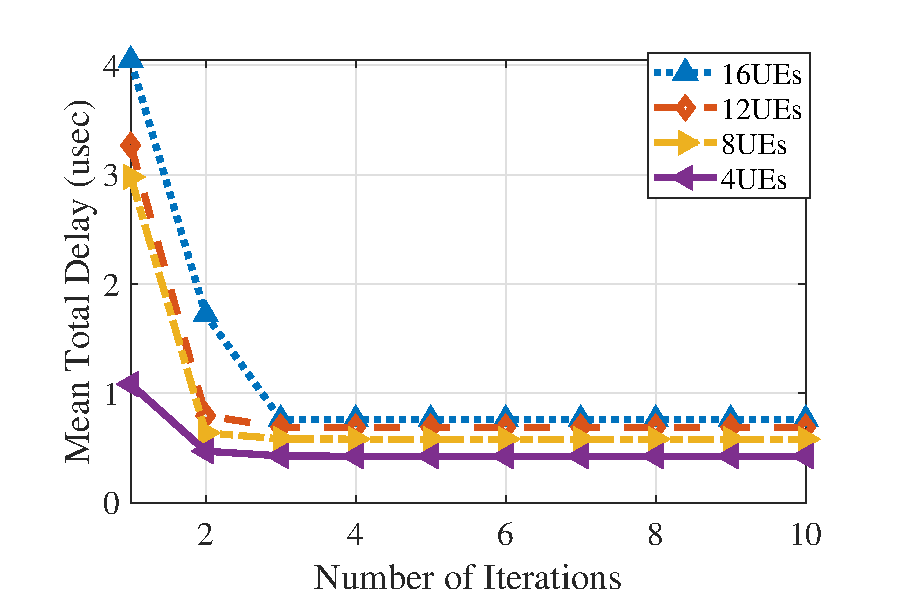
\includegraphics[scale = 0.5]{iterD.eps}
    %\includegraphics[max height=30cm,max width=9.5cm]{Drawing15.eps}
    %\includegraphics[width=\textwidth]{finalDraw.pdf}
  \caption{Mean Total Delay (usec) vs. Number of iterations}
  \label{fig:2}
\end{figure}

Table I shows the execution time versus the number of UEs for one service. We run our simulation on the system with configures (RAM = 8 GB, CPU = Core i5, SSD Hard Disk). 
 As the number of UEs in the system increases, the execution time increases polynomially. 
\begin{table}[H]
\captionsetup{labelformat=empty}
 \caption {Table(I) Execution Time vs. Number of UEs} 
\begin{center}
 \scalebox{0.9}{
\begin{tabular}{|| l || l| l |l |l |l ||}
 \hline
Number of UEs & 5 & 10 & 15 & 20 & 25 \\ 
Execution Time (usec)& 12.156 & 19.156 &  29.140 & 44.573 & 67.912 \\
 \hline
\end{tabular}}
\end{center}
\end{table}


\begin{longtable}{|p{0.975\textwidth}|}
\hline \hline
\RaggedRight
\cellcolor{gray!15}
\textbf{\noindent Comment8:} `As a final remark, the structure of the paper needs major re-construction. Several Sections are very lengthy and could be reduced while creating additional Sections. In the current format it is very hard to follow. ''\\
\hline
\end{longtable}
\vspace*{-1\baselineskip}
\noindent \textbf{Response:\\}
Thank you for this comment to make our paper more readable. We modified the entire paper based on this comment.
We updated the manuscript while creating additional Sections such as "background" and "related literature" Sections. Moreover, we modified and shortened the unnecessary paragraphs, for instance, in the "introduction," "system model," and "numerical results." Our paper was modified totally to satisfy the reviewer's concerns.

\begin{longtable}{|p{0.975\textwidth}|}
\hline \hline
\RaggedRight
\cellcolor{gray!15}
\textbf{\noindent Comment9:} `Moreover, there are some typos in the manuscript. For instance, user equipements: user equipment.  ''\\
\hline
\end{longtable}
\vspace*{-1\baselineskip}
\noindent \textbf{Response:\\}
We appreciate your comment about troubleshooting our paper and removing mistakes. Using this comment as a guide, we modified the entire paper. We revised semantic and grammar problems. We reread our paper and tried to correct mistakes the same as this.

\begin{longtable}{|p{0.975\textwidth}|}
\hline \hline
\RaggedRight
\cellcolor{gray!15}
\textbf{\noindent Comment10:} `Furthermore, some acronyms are not explained in the text e.g., Quality of Service (QoS). ''\\
\hline
\end{longtable}
\vspace*{-1\baselineskip}
\noindent \textbf{Response:\\}
Based on this comment, we added a Table I reporting the list of acronyms to our paper as follow

\begin{table}[H]
\vspace*{-0em}
 \caption {List of Acronyms} \label{table:11a}
 \vspace*{-1em}
 \begin{center}
 \scalebox{1}{
  \begin{tabular}{l  l }
  \toprule
  \vspace*{-0.2em}
\textbf{Acronym} & \textbf{Definition} \\ [0.5ex]
   \toprule
  VNF & virtual network function\\[.5ex]
  
  VM & virtual machine  \\[.5ex]
  RAN &  radio access network \\[.5ex]
 O-RAN & open RAN  \\[.5ex]
 vRAN & virtual RAN \\[.5ex]
 CRAN & cloud RAN \\[.5ex]
   QoS &  quality of service \\[.5ex]
  MIMO & multiple input multiple output \\[.5ex]
  PRB &  physical resource block \\[.5ex]
  SINR & signal to interference and noise ratio  \\[.5ex]
  eMBB & enhanced mobile broadBand \\[.5ex]
  
  URLLC  & ultra-reliable low latency communication \\[.5ex]
   
  mMTC &  massive machine-to-machine communications \\[.5ex]
  
  O-RU &  O-RAN radio unit \\[.5ex]
 
   O-DU &  O-RAN distributed unit \\ [.5ex]
  
   O-CU &  O-RAN central unit \\ [.5ex]
  
     UPF &  user plane function \\ [.5ex]
  
  UE &  user equipment \\ [.5ex]
  SINR & signal-to-noise-plus-interference ratio \\ [.5ex]
  CAPEX & capital expenditures  \\ [.5ex]
  OPEX & operating expenses  \\ [.5ex]
  
  KKT &  Karush-Kuhn-Tucker \\ [.5ex]
 \toprule
 \end{tabular}}
 \end{center}
 \end{table}

\begin{longtable}{|p{0.975\textwidth}|}
\hline \hline
\RaggedRight
\cellcolor{gray!15}
\textbf{\noindent Comment11:} `Finally, the figures in the current version of the manuscript are very small and extremely hard to read. Therefore, re-formatting is necessary. ''\\
\hline
\end{longtable}
\vspace*{-1\baselineskip}
\noindent \textbf{Response:\\}
We modified all figures to make them more readable due to this comment. We enlarge the texts of the figures, bold the lines and markers, and re-formatting all the figures.


\clearpage
\noindent
\begin{longtable}{|p{.975\textwidth}|}
\hline \hline %\hline \hline \hline
\Centering
\cellcolor{gray!60}
\textbf{Reviewer 3} \\
\hline \hline %\hline \hline \hline
\RaggedRight
\cellcolor{violet!15}
\textbf{\noindent Comments to the Author} ``
The reviewer has addressed most of the comments satisfactorily. However, the paper still contains some minor issues as follows ''\\
\hline
\end{longtable}
\vspace*{-1\baselineskip}
\noindent \textbf{Response:\\}
We are pleased to thank the reviewer for his/her detailed and thorough reading of this manuscript. We hope that the responses provided here will assist the reviewer in relieving his or her concerns.

\begin{longtable}{|p{0.975\textwidth}|}
\hline \hline
\RaggedRight
\cellcolor{gray!15}
\textbf{\noindent Comment1:} ``Abbreviations such as QoS, CAPEX and OPEX are not expanded at their first use. ''\\
\hline
\end{longtable}
\vspace*{-1\baselineskip}
\noindent \textbf{Response:\\}
Based on this comment, we added a Table I reporting the list of acronyms to the paper that is shown as below

\begin{table}[H]
\vspace*{-0em}
 \caption {List of Acronyms} \label{table:11a}
 \vspace*{-1em}
 \begin{center}
 \scalebox{1}{
  \begin{tabular}{l  l }
  \toprule
  \vspace*{-0.2em}
\textbf{Acronym} & \textbf{Definition} \\ [0.5ex]
   \toprule
  VNF & virtual network function\\[.5ex]
  
  VM & virtual machine  \\[.5ex]
  RAN &  radio access network \\[.5ex]
 O-RAN & open RAN  \\[.5ex]
 vRAN & virtual RAN \\[.5ex]
 CRAN & cloud RAN \\[.5ex]
   QoS &  quality of service \\[.5ex]
  MIMO & multiple input multiple output \\[.5ex]
  PRB &  physical resource block \\[.5ex]
  SINR & signal to interference and noise ratio  \\[.5ex]
  eMBB & enhanced mobile broadBand \\[.5ex]
  
  URLLC  & ultra-reliable low latency communication \\[.5ex]
   
  mMTC &  massive machine-to-machine communications \\[.5ex]
  
  O-RU &  O-RAN radio unit \\[.5ex]
 
   O-DU &  O-RAN distributed unit \\ [.5ex]
  
   O-CU &  O-RAN central unit \\ [.5ex]
  
     UPF &  user plane function \\ [.5ex]
  
  UE &  user equipment \\ [.5ex]
  SINR & signal-to-noise-plus-interference ratio \\ [.5ex]
  CAPEX & capital expenditures  \\ [.5ex]
  OPEX & operating expenses  \\ [.5ex]
  
  KKT &  Karush-Kuhn-Tucker \\ [.5ex]
 \toprule
 \end{tabular}}
 \end{center}
 \end{table}
\begin{longtable}{|p{0.975\textwidth}|}
\hline \hline
\RaggedRight
\cellcolor{gray!15}
\textbf{\noindent Comment2:} ``Eq. (3) includes inter-slice interference but a sentence following the equation mentions that there is no inter-slice interference because slices are isolated, which is confusing''\\
\hline
\end{longtable}
\vspace*{-1\baselineskip}
\noindent \textbf{Response:\\} 
We thank the reviewer for reporting this ambiguity.
We revised this section, rewrote the equation (3), by removing the inter-slice interference to clarify this equation. Moreover, we removed two figures of Fig. 2 and Fig. 3 since they don't add much to what is already written in words, and even Fig. 2 makes the paper vaguer, and we also aim for a more concise manuscript.
Below we report the revised sentences.
 
Network slicing techniques significantly reduce inter-service (inter-slice) interference.
One way consists in leveraging a two-time scale PRB scheduling to isolate PRBs in slices (in the first time scale) and schedule the PRBs to the UEs of the slices (in the second time scale). Another method consists of allocating part of the PRBs of eMBB services to URLLC and mMTC [2], [5], [32]. In this paper, we assume that the PRB scheduling is performed. Also, in Section V-A, we briefly study the PRB scheduling between slices.
Since there are limited resources, inter-service interference cannot be eliminated entirely. Nevertheless, isolating the slices reduces inter-service interference considerably and allows us to ignore it mathematically.
Back to \eqref{eq1}, $I_{r,u(s,i)}^{k}$ is the sum of the power of interfering signals and quantization noise, and can be represented as 
%{\color{red} use paranthesis in the following equation to clear +}
%\begin{subequations}\label{eqI}
%\begin{alignat}{4}
%\begin{align}\label{eqI}
%&I_{r,u(s,i)}^{k} =\nonumber\\
% &\underbrace{\sum_{\substack{l=1 \\ l\neq i}}^{{U}_{s}} e^{k}_{u(s,i)}e^{k}_{u(s,l)}  p_{u(s,l)}^{k}\sum_{\substack{r'=1 \\ r'\neq r}}^{R}|{\bold{h}_{r',u(s,i)}^{k \: H}} \bold{w}_{r',u(s,l)}^{k} g_{u(s,l)}^{r'}|^2}_{\text{(intra-slice interference)}}+\nonumber\\
%&\underbrace{\sum_{\substack{n = 1 \\ n\neq s}}^{S}\sum_{l=1}^{{U}_s} e^{k}_{u(s,i)}e^{k}_{u(n,l)}  p_{u(n,l)}^{k}\sum_{\substack{r'=1 \\ r'\neq r}}^{R}|{\bold{h}_{r',u(s,i)}^{k \: H}} \bold{w}_{r',u(n,l)}^{k} g_{u(n,l)}^{r'}|^2}_{\text{(inter-slice interference)}}\nonumber\\
%&+\underbrace{  \sum_{j=1}^{{R}} {\sigma_q}^2 |\boldsymbol{h}_{r,{u(s,i)}}^k|^2 }_{\text{(quantization noise)}},
%\end{align}
%\end{alignat}
%\end{subequations}
%{\color{red} $\gamma_1$ is constant used instead of variable. }
\begin{align}\label{eqI}
&I_{r,u(s,i)}^{k} =+\underbrace{  \sum_{j=1}^{{R}} {\sigma_q}^2 |\boldsymbol{h}_{r,{u(s,i)}}^k|^2 }_{\text{(quantization noise)}}\nonumber\\
 &\underbrace{\sum_{\substack{l=1 \\ l\neq i}}^{{U}_{s}} e^{k}_{u(s,i)}e^{k}_{u(s,l)}  p_{u(s,l)}^{k}\sum_{\substack{r'=1 \\ r'\neq r}}^{R}|{\bold{h}_{r',u(s,i)}^{k \: H}} \bold{w}_{r',u(s,l)}^{k} g_{u(s,l)}^{r'}|^2}_{\text{(intra-slice interference)}},
\end{align}
%where $\gamma_{1} = e^{k}_{u(s,i)}e^{k}_{u(s,l)}$ and $\gamma_{2} = e^{k}_{u(s,i)}e^{k}_{u(n,l)}$.
where $e^{k}_{u(s,i)}$ is a binary variable that indicates whether the $k^{th}$ PRB is allocated to the UE $i$ in slice $s$, assigned to $r^{th}$ O-RU, or not. %($\gamma_1$ and $\gamma_2$ are two variales. You  define on variable here.)
Furthermore, there is no inter-slice interference, only intra-slice interference, since slices are assumed to be isolated. 
\begin{longtable}{|p{0.975\textwidth}|}
\hline \hline
\RaggedRight
\cellcolor{gray!15}
\textbf{\noindent Comment3:} ``The captions of Figs. 9, 12 and 14 are incomplete.''\\
\hline
\end{longtable}
\vspace*{-1\baselineskip}
\noindent \textbf{Response:\\}  
Thank you for this comment. We checked and corrected all the figure's captions.

\begin{longtable}{|p{0.975\textwidth}|}
\hline \hline
\RaggedRight
\cellcolor{gray!15}
\textbf{\noindent Comment4:} ``It is recommended to discuss each result figure in one paragraph. Currently, the discussions on Figs. 5-11 are packed into one paragraph, which is difficult to read.''\\
\hline
\end{longtable}
\vspace*{-1\baselineskip}
\noindent \textbf{Response:\\}  
We would like to thank the reviewer for reducing the ambiguity of our paper with this comment. Each figure was discussed as an individual paragraph in response to this comment.

\begin{longtable}{|p{0.975\textwidth}|}
\hline \hline
\RaggedRight
\cellcolor{gray!15}
\textbf{\noindent Comment5:} ``Another round of proofread is required, as there are some mathematical variables which are not italicized and some sentences are incomplete.''\\
\hline
\end{longtable}
\vspace*{-1\baselineskip}
\noindent \textbf{Response:\\}  
We modified the whole paper based on this comment, tried correcting all mathematical variables, and revised all sentences again. We checked all the system model and proposed algorithms and corrected the italicized text and vice versa. For instance, we corrected the $\log$, $\max$, and $\min$ and other texts that are written in italics. Moreover, we italicized variables that were written in non-italicized.
\end{document}


